
\section{Results}
\label{sec:results}


We evaluate \sysname on end-to-end quality (\cref{sec:e2e}),
training FLOP scaling (\cref{sec:train-scaling}), and test-time scaling
(\cref{sec:inf-scaling}). We find that \sysname outperforms both parameter-
and data-matched RDMs and Transformers, optimal looping and data
follow predictable power laws, and test-time looping follows a saturating exponential decay.

\begin{table*}[!t]
    \centering
    \small
    \setlength{\tabcolsep}{4pt}
    \renewcommand{\arraystretch}{1.05}
    \begin{tabular*}{\textwidth}{@{\extracolsep{\fill}} llccc|ccccccc @{}}
        \toprule
         & \textbf{Model} & $\mathbf{T}$ & Val. & WikiText & Hellaswag & ARC-c & ARC-e & PIQA & BoolQ & SciQ & Avg. \\
         \midrule
         \multirow{2}{*}{\rotatebox{90}{100M}}
         & RDM& 16 & 14.23 & 63.27 & 27.16 & 17.66 & 42.38 & 59.14 & 51.35 & \textbf{72.50} & 45.03 \\
         & \sysname & 16 & \textbf{13.59} & \textbf{60.33} & \textbf{27.18} & \textbf{18.09} & \textbf{43.10} & \textbf{59.30} & \textbf{61.83} & 71.50 & \textbf{46.83} \\
        \midrule
         \multirow{2}{*}{\rotatebox{90}{350M}}
         & RDM& 8  & 10.76 & 41.31 & 28.55 & 20.90 & 47.26 & 61.75 & \textbf{61.53} & 76.70 & 49.45 \\
         & \sysname & 8  & \textbf{10.09} & \textbf{37.53} & \textbf{29.23} & \textbf{21.08} & \textbf{48.78} & \textbf{62.08} & 60.73 & \textbf{78.80} & \textbf{50.12} \\
         \bottomrule
    \end{tabular*}
    \caption{\textbf{Zero-Shot and Perplexity Results Trained on RDM Setup.} Comparison of \sysname and RDM \citep{geiping_scaling_2025} on 
    a variety of open source benchmarks and perplexity held-out validation set and Wikitext \citep{merity2016pointer}. \textbf{Best} results are \textbf{bolded}.}
    \label{tab:rdm-parcae}
\end{table*}


\begin{table}[!t]
\centering
\small
\setlength{\tabcolsep}{4.5pt}
\begin{tabular}{l ccc ccc ccc}
\toprule
& \multicolumn{3}{c}{Val Loss ($\downarrow$)} & \multicolumn{3}{c}{Core ($\uparrow$)} & \multicolumn{3}{c}{Core Ext ($\uparrow$)} \\
\cmidrule(lr){2-4} \cmidrule(lr){5-7} \cmidrule(lr){8-10}
Configuration & $T\!=\!1$ & $T\!=\!4$ & $T\!=\!8$ & $T\!=\!1$ & $T\!=\!4$ & $T\!=\!8$ & $T\!=\!1$ & $T\!=\!4$ & $T\!=\!8$ \\
\midrule
RDM          & \multicolumn{3}{c}{\textit{Divergent Training}} & \multicolumn{3}{c}{\textit{Divergent Training}} & \multicolumn{3}{c}{\textit{Divergent Training}}\\
+\,Constrained\ $\dA$       & 8.99 & 3.15 & 2.97 & $-2.0_{\pm0.1}$ & $11.0_{\pm0.1}$ & $13.2_{\pm0.2}$ & $0.5_{\pm0.1}$ & $7.8_{\pm0.0}$ & $9.1_{\pm0.5}$ \\
+\,Per-Seq.\ Sampling & 3.38 & 3.01 & 2.98 & $\mathbf{7.6_{\pm0.2}}$ & $13.4_{\pm0.2}$ & $14.0_{\pm0.2}$ & $\mathbf{5.9_{\pm0.4}}$ & $9.3_{\pm0.2}$ & $\mathbf{9.9_{\pm0.2}}$ \\
+\,Prelude Norm       & \textbf{3.28} & \textbf{2.97} & \textbf{2.95} & $7.5_{\pm0.3}$ & $\mathbf{13.5_{\pm0.0}}$ & $\mathbf{14.0_{\pm0.2}}$ & $5.8_{\pm0.3}$ & $\mathbf{9.4_{\pm0.1}}$ & $9.7_{\pm0.3}$ \\
\bottomrule
\end{tabular}
\caption{\textbf{Stability Results Trained on Transformer Setup.} To illustrate stability, we retrofit a baseline 140M Transformer into a RDM and then sequentially add our stability improvements.}
\label{tab:ablation}
\end{table}



\subsection{\sysname Improves End-to-End Quality}
\label{sec:e2e}

We compare \sysname against parameter- and data-matched RDMs and Transformers, finding that \sysname is more stable than prior looped models and that it outperforms both in quality. 

\paragraph{Setup.} 
For RDMs, we follow \citet{geiping_scaling_2025}, using the Huginn dataset and tokenizer for training. For transformers, we follow \citet{nanochat} and train on \texttt{FineWeb-Edu} \citep{penedo2024finewebdatasetsdecantingweb}.
For both RDM and Transformer setups, we perform hyperparameter sweeps for both RDMs and Transformers, and then use them for \sysname (i.e., we perform no hyperparameter sweeps for \sysname models). Extended model definitions, hyperparameter selection, and evaluation setup can be found in \cref{sec:model-definitions}, \cref{sec:hyperparameters}, and \cref{sec:evaluation-setup}, respectively. 

\textbf{Comparison against RDMs}. \cref{tab:rdm-parcae} shows that \sysname reduces perplexity by up to 6.2 \% and 9.1 \% on a held-out validation set and WikiText \citep{merity2016pointer} against prior RDMs \citep{geiping_scaling_2025}, while additionally performing up to 1.8 points better on the average of several downstream benchmarks. \cref{tab:ablation} ablates that each modification of \sysname contributes:
constraining $\dA$ enables convergence at high $T$ (e.g., $\mu_{\text{rec}}=T\!=\!8$),
per-sequence sampling stabilizes lower test-time depths, and the prelude norm
further improves quality across all $T$ (and late stage stability \cref{sec:prelude-norm}).






\begin{table*}[!t]
    \centering
    \small
    \setlength{\tabcolsep}{4pt}
    \renewcommand{\arraystretch}{1.05}
    \begin{tabular*}{\textwidth}{@{\extracolsep{\fill}} llc|cccc @{}}
        \toprule
         & \textbf{Model} & $\mathbf{T}$ & Val. PPL ($\downarrow$) & Lambada PPL ($\downarrow$) & Core ($\uparrow$) & Core-Extended ($\uparrow$) \\
        \midrule
        \multirow{2}{*}{\rotatebox{90}{140M}} & Transformer & -- & 21.48 & 127.39 & 13.00 ± 0.15 & 8.80 ± 0.21 \\
         & \sysname & 8  & \textbf{19.06} & \textbf{80.64} & \textbf{14.04 ± 0.20} & \textbf{9.67 ± 0.28} \\
        \midrule
        \multirow{2}{*}{\rotatebox{90}{370M}} & Transformer & -- & 15.79 & 40.77 & 17.46 ± 0.03 & 11.71 ± 0.22 \\
         & \sysname & 8  & \textbf{14.49} & \textbf{32.74} & \textbf{20.00 ± 0.06} & \textbf{12.75 ± 0.31} \\
        \midrule
        \multirow{2}{*}{\rotatebox{90}{770M}} & Transformer & -- & 13.08 & 22.37 & 22.42 ± 0.20 & 14.20 ± 0.63 \\
         & \sysname & 8  & \textbf{12.49} & \textbf{19.71} & \textbf{25.07 ± 0.33} & \textbf{15.19 ± 0.43} \\
        \midrule
        \multirow{2}{*}{\rotatebox{90}{1.3B}} & Transformer & -- & 11.95 & 17.26 & 25.45 ± 0.08 & 15.90 ± 0.23 \\
         & \sysname & 8  & \textbf{11.42} & \textbf{14.71} & \textbf{28.44 ± 0.28} & \textbf{17.08 ± 0.09} \\
        \bottomrule
    \end{tabular*}
    \caption{\textbf{Comparing \sysname to Fixed-Depth Transformers.} We pretrain Transformers and \sysname with a \texttt{nanochat} setup at several scales, evaluating on a held-out validation set, Lambada \citep{paperno2016lambada}, Core, and Core-Extended \citep{li2025datacomplmsearchgenerationtraining}. 
    \textbf{Best} results are \textbf{bolded.}}
    \label{tab:trans-parcae}
\end{table*}


\textbf{Comparison Against Transformers.} \cref{tab:trans-parcae} shows that \sysname reduces validation perplexity by 4.3--9.2\% and improves Core and Core-Extended Scores by up to 2.99 and 1.18 points, respectively. We find that our 770M \sysname model achieves quality comparable to the 1.3B Transformer on Core \citep{li2025datacomplmsearchgenerationtraining} with roughly half the parameters. 
Measured as a fraction of the quality gap to the next larger Transformer (e.g., for 140M Core-Extended: $\frac{9.67-8.80}{11.71-8.80} \cdot 100 \approx 29.9 \%$), \sysname achieves a \textbf{\emph{23.3-87.5\% and 29.9-58.2\%}} better parameter efficiency for Core and Core-Extended, respectively.





\begin{figure}[!t]
    \centering
    \vspace{-0.4em}
    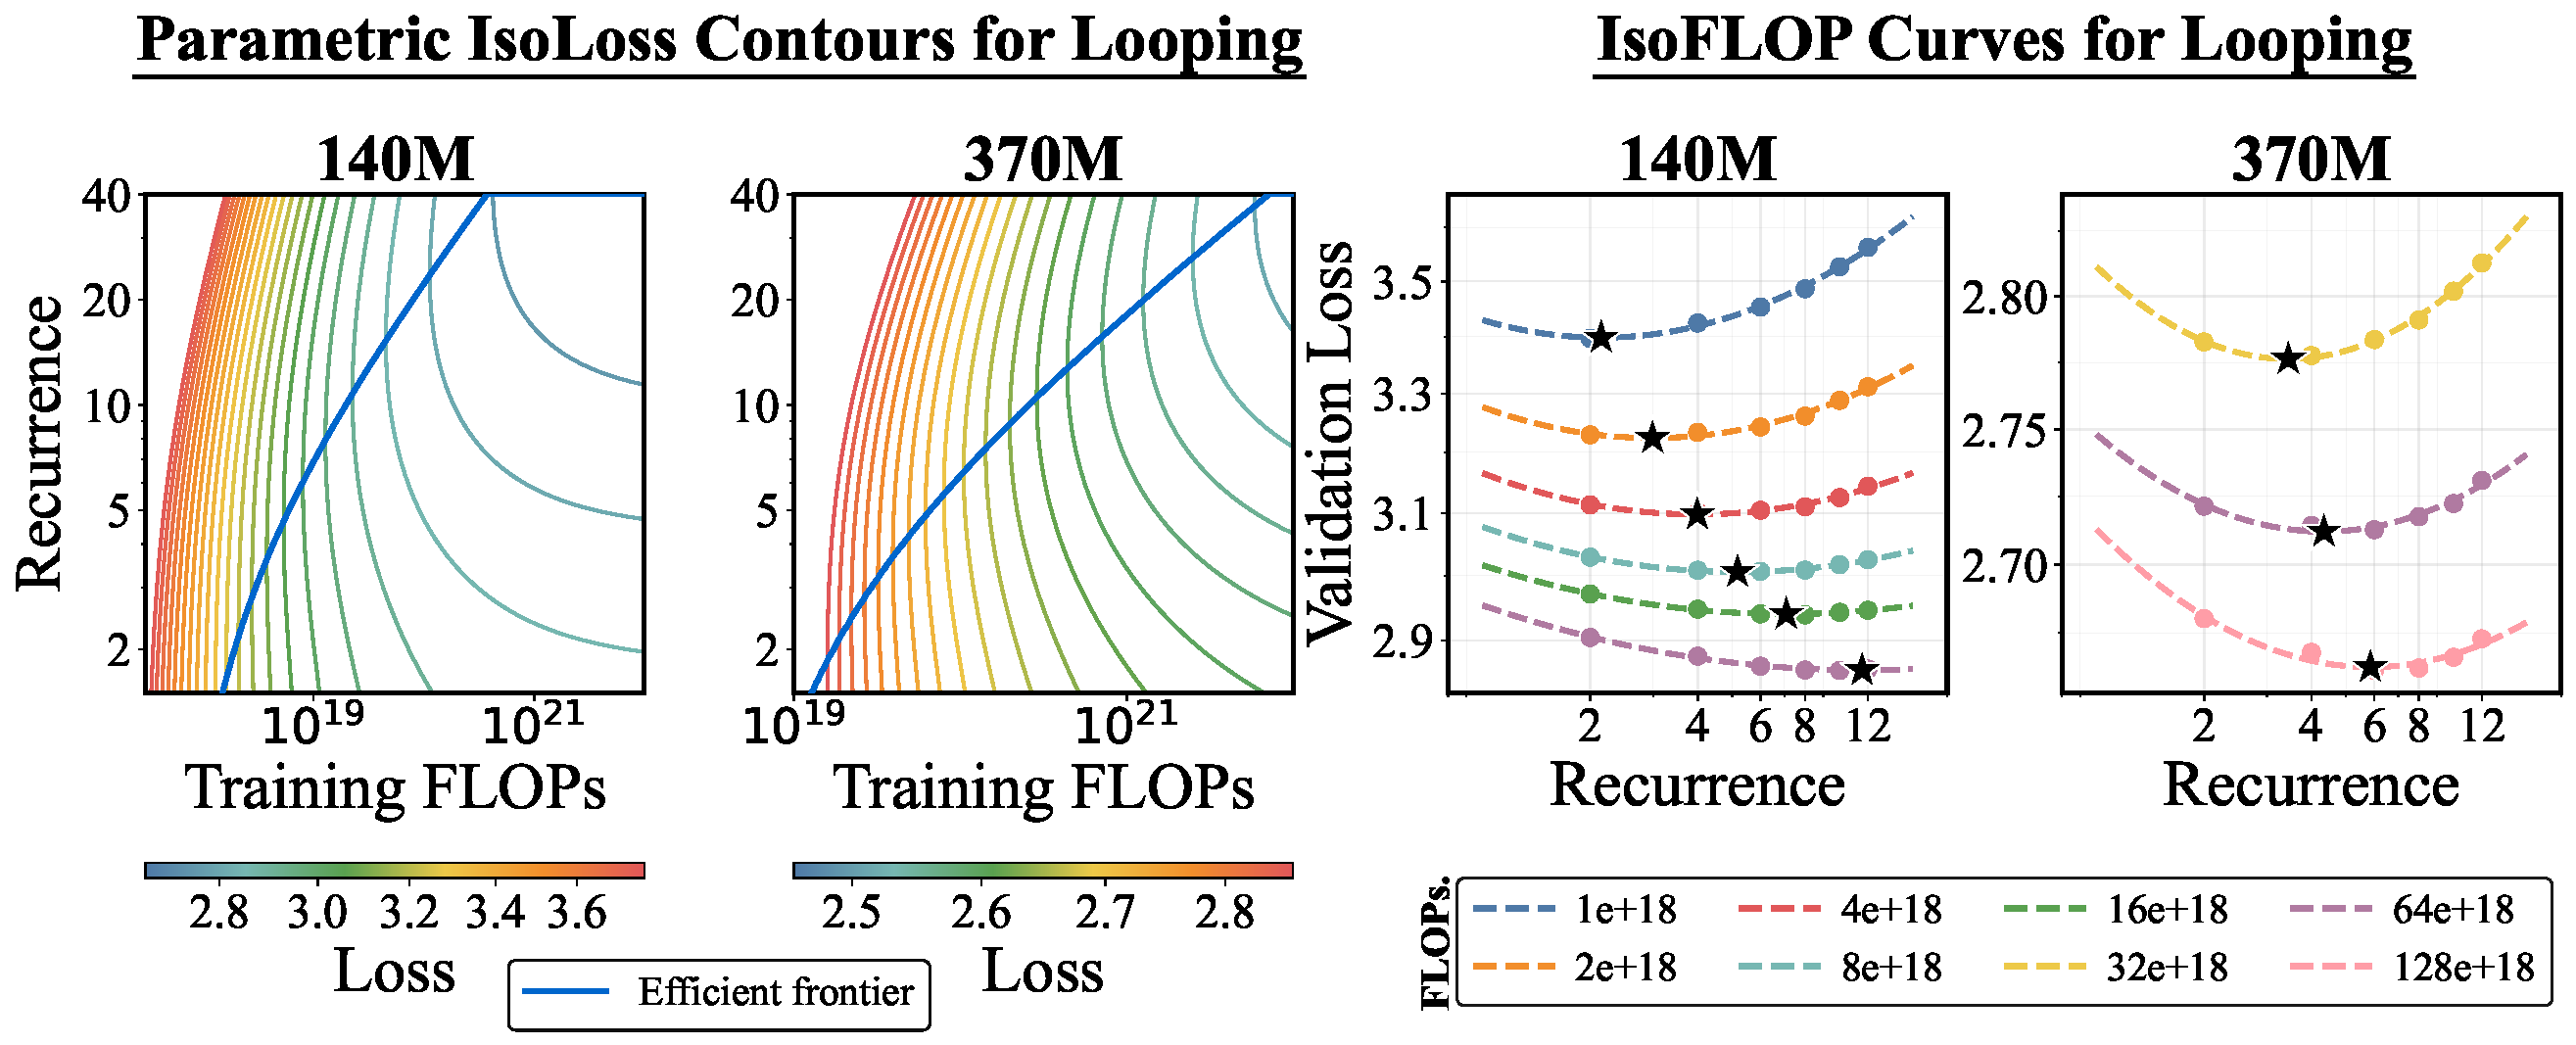
\includegraphics[width=\linewidth]{figures/main/combined_contours_isoflop.pdf}
    \vspace{-1.4em}
    \caption{\textbf{Looping Scales Training Compute Optimally.}~(\emph{Left}) Parametric isoLoss contours over \meanrecurrence and data. The efficient frontier (blue line) traces the lowest FLOP budget required to achieve each loss level, showing that optimal training requires increased looping. (\emph{Right}) Parabolic isoFLOP fits for 140M and 370M models reveal a clear optimum \meanrecurrence at each FLOP budget, indicating that looping is an orthogonal scaling axis to data.}
    \label{fig:train-scaling-laws}
    \vspace{-0.4em}
\end{figure}


\subsection{Looping as an Orthogonal Scaling Axis in Training}
\label{sec:train-scaling}

In this section, we explore the FLOP efficiency of looping under a fixed FLOP and parameter budgets. We find that looping introduces an orthogonal axis for scaling compute, where compute-optimal training increases \meanrecurrence and data in tandem following empirical power laws.

\paragraph{Setup.} We train 140M and 370M \sysname models under fixed FLOP and parameter budgets, varying training tokens and mean recursion \meanrecurrence using the \texttt{nanochat} setup. Additional training details and FLOP estimates can be found in \cref{sec:scaling-laws-setup} and \cref{sec:flop-estimate}, respectively.

\textbf{Modeling Scaling Laws of Looping}. At 140M and 370M scales, isoFLOP curves show that increasing \meanrecurrence while proportionally reducing tokens yields lower validation loss than training at low recurrence (\cref{fig:train-scaling-laws} [\emph{right}]). Using a parabolic fit, we extract the optimal \meanrecurrence and token budget at each FLOP level, finding that both follow predictable power laws (\cref{fig:power-laws}) with consistent exponents ($\gamma_{\mu} \approx 0.40$, $\gamma_D \approx 0.78$). 
We also fit a parametric function $\widehat{\mathcal{L}}(\mu_{\text{rec}}, D) = E + X\cdot \mathbf{N}(\mu_{\text{rec}})^{-x} + Y \cdot D^{-y}$ over the effective parameterization $\mathbf{N}(\mu_{\text{rec}})$ (i.e., parameters of unrolling the looped model) and tokens $D$ (\cref{fig:train-scaling-laws}, [\emph{left}]; details in \cref{sec:fit-par}), enabling predictable extrapolation of loss to unseen budgets. To verify, we predict the validation loss of held-out models in \cref{sec:e2e}, achieving 1.3\% and 0.8\% error at 140M and 370M, respectively.


\begin{figure}[!t]
    \centering
    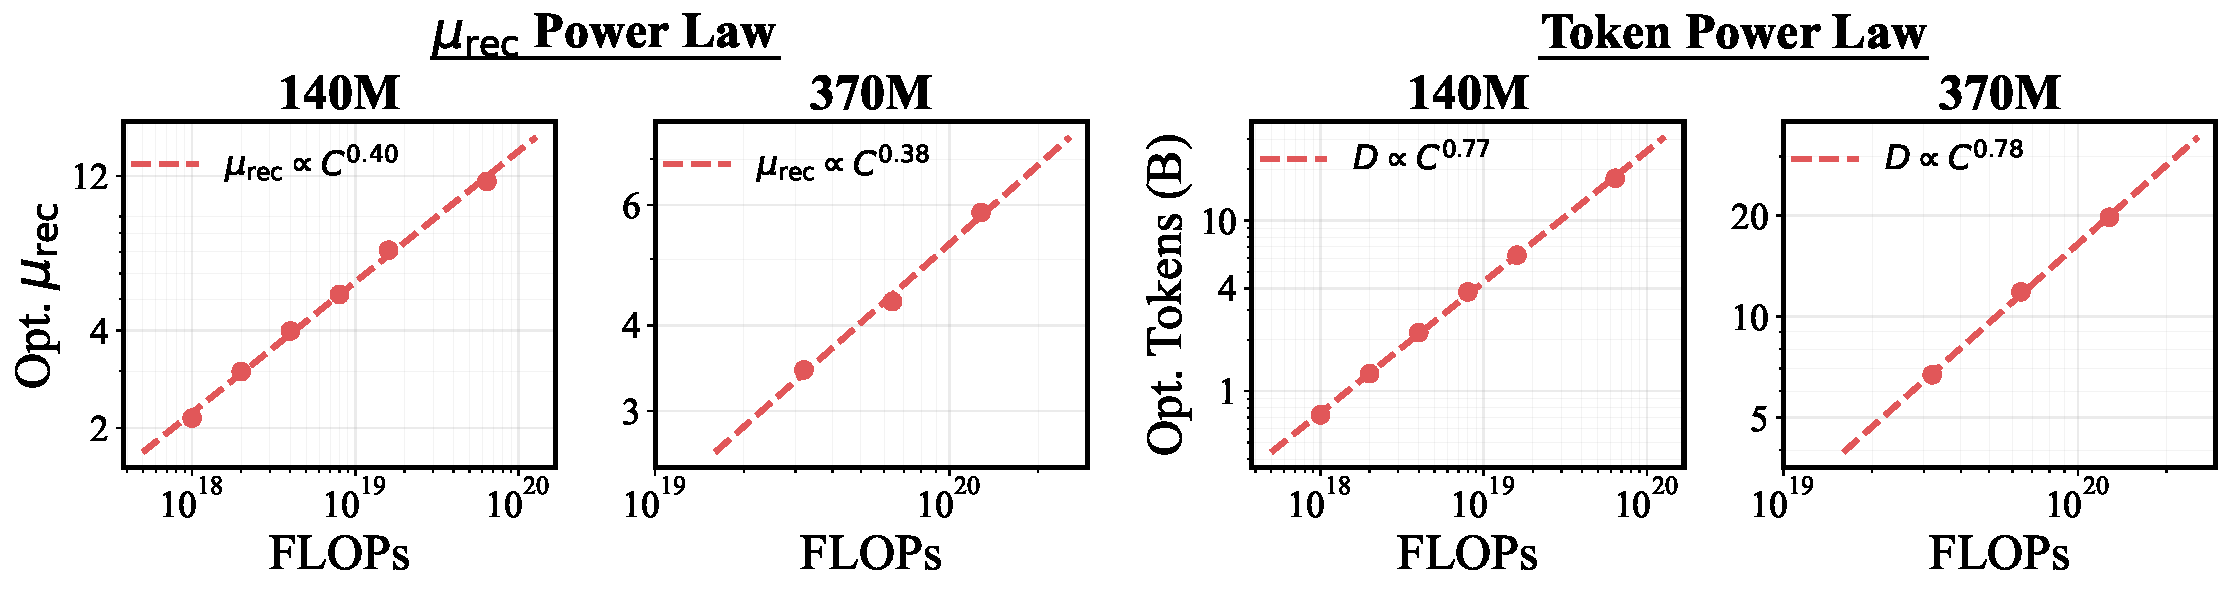
\includegraphics[width=\linewidth]{figures/main/optimal_recurrence_data_combined.pdf}
    \vspace{-1.5em}
    \caption{\textbf{Optimal \meanrecurrence and Tokens Follows Predictable Power Laws.} We fit a parabola to each isoFLOP budget for both 140M and 370M \sysname models, using its minima to approximate the optimal \meanrecurrence and token budget at each scale. We observe that optimal recurrence (\emph{left plots}) and tokens (\emph{right plots}) follow a predictable power law with similar coefficients at both scales.}
    \label{fig:power-laws}
\end{figure}


\begin{table}[!t]
    \centering
    \begin{minipage}[t]{0.38\textwidth}
        \vspace{-6pt}
        \centering
        \makeatletter\def\@captype{figure}\makeatother
        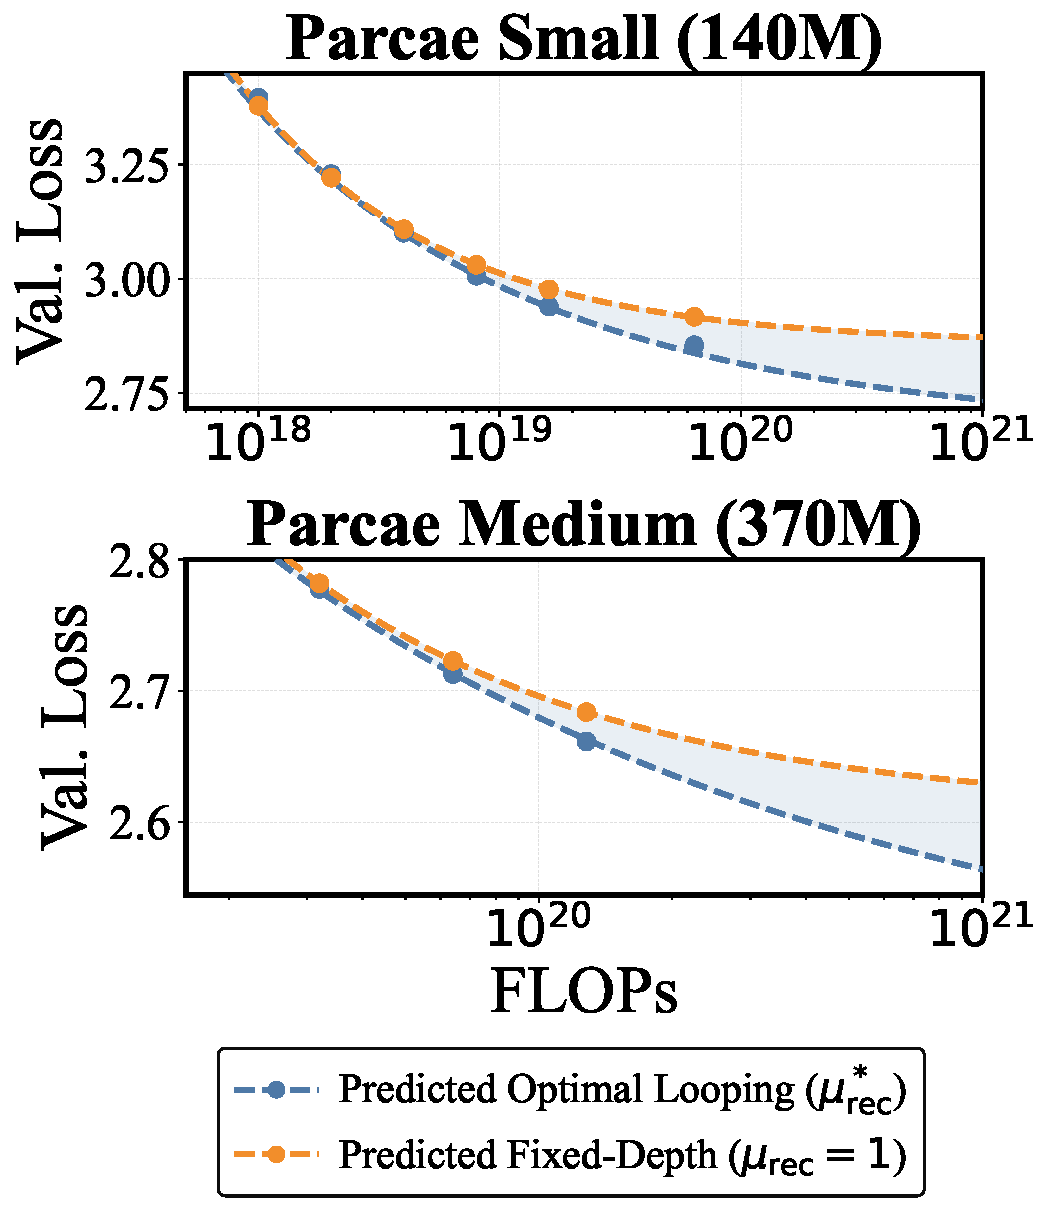
\includegraphics[width=\linewidth]{figures/main/frontier_vs_rec1_fit.pdf}
        \vspace{-1.56em}
        \caption{\textbf{Pareto Frontier of Looping.} We observe that looping has a stricter IsoFLOP optimal loss frontier over fixed-depth, non-looped models. Dots are empirical points.}
        \label{fig:optimal-frontier}
    \end{minipage}
    \hfill
    \begin{minipage}[t]{0.60\textwidth}
        \vspace{0pt}
        \centering
        \begin{tabular}{@{}c cc | cc | cc@{}}
        \toprule
        & \textbf{FLOPs}& & \multicolumn{2}{c}{\textbf{Optimal $\mu_{\mathrm{rec}}^*$}} & \multicolumn{2}{c}{\textbf{Fixed-Depth}} \\
        \cmidrule(lr){4-5} \cmidrule(lr){6-7}
        & ($\times 10^{18})$ & $\mu_{\mathrm{rec}}^*$ & Core & Core Ext. & Core & Core Ext. \\
        \midrule
        \multirow{6}{*}{\rotatebox[origin=c]{90}{\textbf{140M}}}
        & $1$   & 2  & $7.6$ & $5.7$ & $\mathbf{7.9}$ & $\mathbf{6.1}$ \\
        & $2$   & 2  & $9.0$ & $6.2$ & $\mathbf{10.5}$ & $\mathbf{6.4}$ \\
        & $4$   & 4  & $\mathbf{11.2}$ & $\mathbf{8.4}$ & $10.7$ & $8.1$ \\
        & $8$   & 6  & $10.5$ & $\mathbf{7.8}$ & $\mathbf{11.8}$ & $7.7$ \\
        & $16$  & 8  & $\mathbf{14.6}$ & $\mathbf{9.8}$ & $13.0$ & $8.8$ \\
        & $64$  & 10 & $\mathbf{16.2}$ & $\mathbf{11.0}$ & $15.0$ & $9.5$ \\
        \midrule
        \multirow{3}{*}{\rotatebox[origin=c]{90}{\textbf{370M}}}
        & $32$  & 4  & $15.2$ & $10.1$ & $\mathbf{16.8}$ & $\mathbf{11.2}$ \\
        & $64$  & 6  & $\mathbf{18.1}$ & $11.6$ & $\mathbf{18.1}$ & $\mathbf{12.1}$ \\
        & $128$ & 6  & $\mathbf{20.1}$ & $\mathbf{13.0}$ & $18.1$ & $12.0$ \\
        \bottomrule
        \end{tabular}
        \caption{\textbf{Core Scores Comparison of Looping Optimal Frontier over Purely Scaling Data.} We evaluate the downstream quality of fixed-depth (\meanrecurrence=1) and looped \sysname models trained with fixed parameters and FLOP budgets. At both scales, using the optimal \meanrecurrence results in better Core and Core-Extended scores at extended FLOP budgets. Expanded results can be found in \cref{sec:fixed-comparison-expanded}.}
        \label{tab:qual-fix-loop}
    \end{minipage}
    \vspace{-1em}
\end{table}


\textbf{IsoFLOP comparison of Looping with Fixed-Depth} \cref{fig:optimal-frontier} shows fixed-depth \sysname models without looping at each FLOP budget. The optimal curve achieves a strictly lower loss, which translates to 1.2-2.0 points higher Core scores (\cref{tab:qual-fix-loop}).







\subsection{Test-Time Scaling Laws of \sysname}
\label{sec:inf-scaling}

We study looping as a mechanism for scaling test-time compute. We find the test-time compute follows a predictable saturating exponential decay, which can be unified with \cref{sec:train-scaling}, connecting both training and test-time scaling laws.

\paragraph{Setup.} We train 140M and 370M \sysname models under a fixed data budget with $\mu_{\text{rec}} \in \{2, 4, 6, 8, 10, 12\}$ following our \texttt{nanochat} setup, evaluating up to $T = 24$. We additionally evaluate models from \cref{sec:train-scaling} for the unified scaling laws. See \cref{sec:scaling-laws-setup} for details.



\textbf{Saturation of Test-Time Compute.} While prior works observed test-time generalization in small synthetic tasks \citep{yangLoopedTransformersAre2023, bansalEndtoendAlgorithmSynthesis2022}, we find quality to be bounded in large-scale language modeling. 
Evaluating models from \cref{sec:e2e} at $2\times$ \meanrecurrence across all four scales (\cref{fig:parcae-test-time-scaling}), we observe that gains plateau near \meanrecurrence, suggesting training depth determines the test-time scaling ceiling.



\begin{figure}[!t]
    \centering
    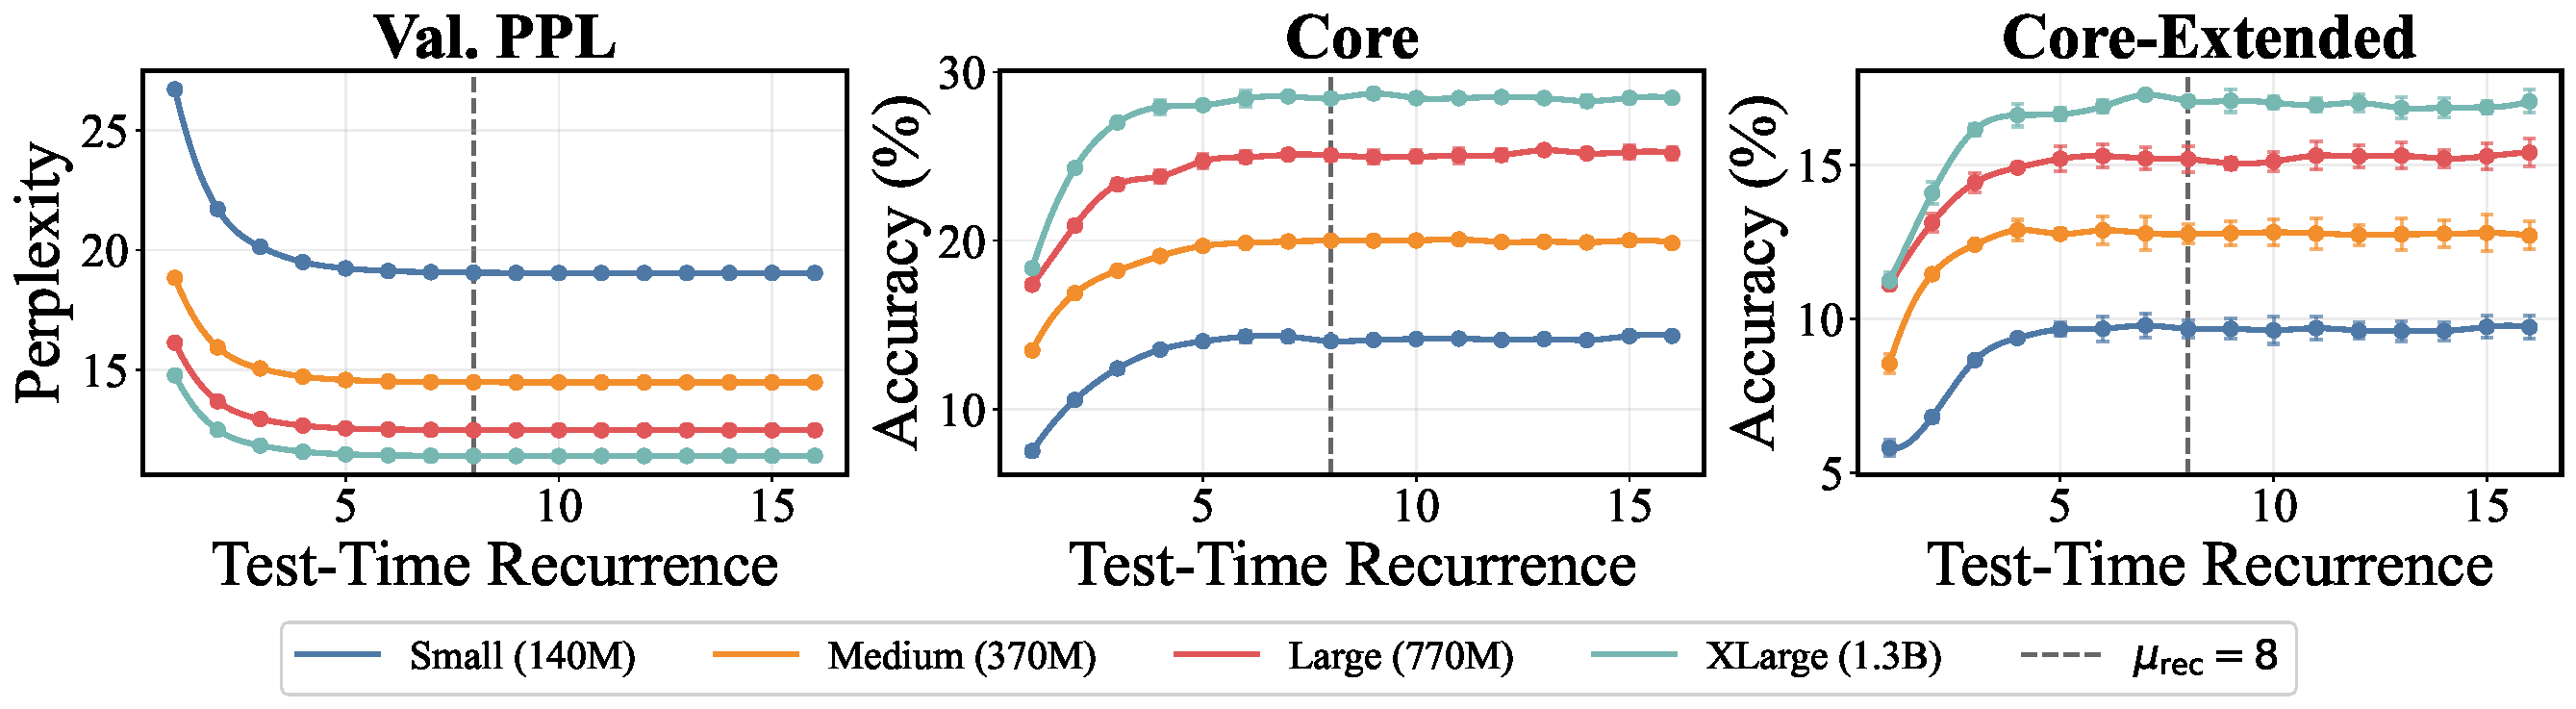
\includegraphics[width=\linewidth]{figures/main/test_time_scaling.pdf}
    \vspace{-1.5em}
    \caption{\textbf{Test-Time Scaling of \sysname.} When evaluating \sysname models from \cref{tab:trans-parcae}, we observe test-time looping follows a predictable saturating trend, consistent across model sizes.}
    \label{fig:parcae-test-time-scaling}
\end{figure}

\begin{figure}[!t]
    \centering
    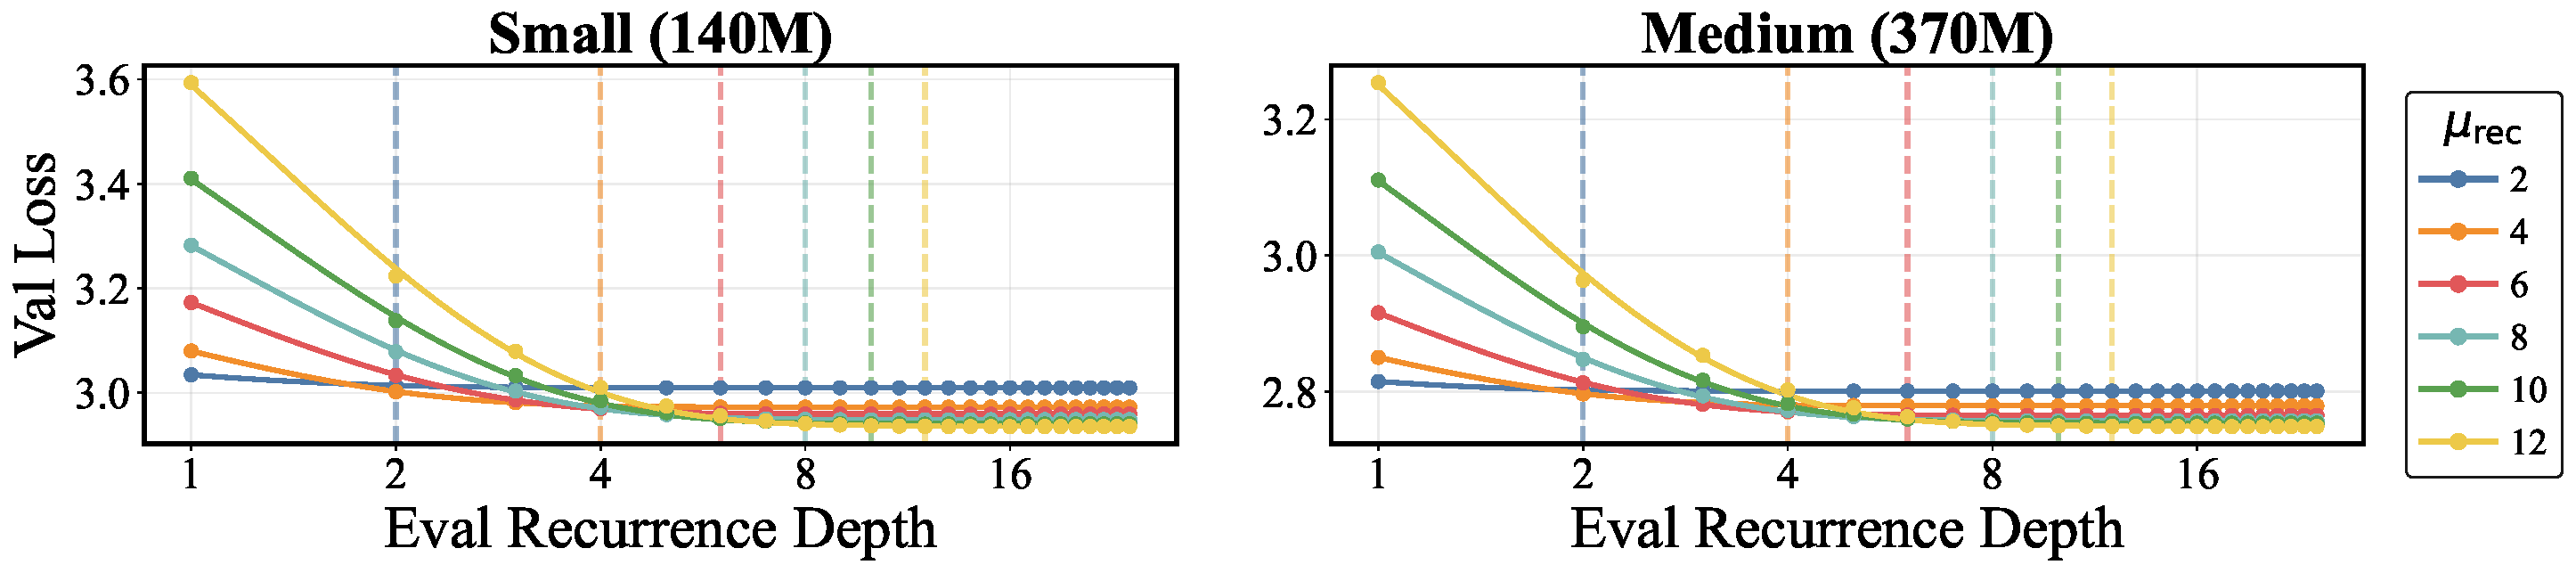
\includegraphics[width=\linewidth]{figures/main/unified_test_time_fixed_tokens_exp_default_tab10.pdf}
    \vspace{-1.4em}
    \caption{\textbf{Scaling Test-Time Compute follows a Predictable Power Laws.}  We plot the validation loss with different \meanrecurrence as a function of test-time recurrence $T$, and find the fitted exponential decay (solid curve for each \meanrecurrence) tightly captures the test-time performance of looping.
    }
    \vspace{-1em}
    \label{fig:test-time-scaling-laws}
\end{figure}

\textbf{Modeling Scaling Laws of Test-Time Looping.} We find that the test-time scaling curves are well-described by a saturating exponential decay of the form: $\mathcal{L}(T) = \mathcal{L}_\infty + Ze^{-z\cdot T}$. This form tightly captures the saturation dynamics for each model (\cref{fig:test-time-scaling-laws}; see \cref{sec:test-par} for details), achieving an average Huber loss of $2.5 \times 10^{-7}$ and $1.8 \times 10^{-7}$ for 140M and 370M, respectively.






\textbf{Unifying Training and Test-Time Scaling Laws.} From the learned fits in \cref{fig:test-time-scaling-laws}, we observe that $\mathcal{L}_\infty$ matches the training law prediction at $T = \mu_\text{rec}$ (\cref{sec:train-scaling}), and that the per-curve decay rate scales inversely with training depth as $z / \mu_\text{rec}$ (see \cref{sec:test-par} for details).
These observations motivate a unified scaling law that connects training and test-time compute:
\begin{equation}
   \widehat{\mathcal{L}}_\text{unified}(T \mid \mu_\text{rec}, D) = \underbrace{E + X \cdot \mathbf{N}(\mu_\text{rec})^{-x} + Y \cdot D^{-y}}_{\text{Training Law Floor } \widehat{\mathcal{L}}_\text{train}(\mu_\text{rec}, D)} + \underbrace{Z \cdot \exp\!\left(-z \cdot T \cdot \mu_\text{rec}^{-1}\right)}_{\text{Test-Time Decay}}
   \label{eq:unified}
\end{equation}
where $\widehat{\mathcal{L}}_{\text{train}}(\mu_{\text{rec}}, {D})$ is the training law in \cref{sec:train-scaling}, and $(Z, z)$ are two fitted parameters governing the test-time scaling. 
The training law sets the irreducible floor, while the decay rate $-z \cdot T / \mu_\text{rec}$ captures how quickly additional recurrences approach it. 
On held-out 140M and 370M \sysname models (\cref{sec:e2e}), the unified fit predicts test-time loss within 0.85-1.31\% average error, dropping further to 0.1-0.17\% average error when the empirical loss at $T = \mu_{\text{rec}}$ is used. This confirms that \cref{eq:unified} captures saturation dynamics, with residual error attributable to the training law's $\sim1\%$ extrapolation gap (see \cref{sec:test-par} for extended details).











